\ccUserChapter{3D Surface Mesh Generation\label{chapter_SurfaceMesher}}
\ccChapterAuthor{Laurent Rineau \and Mariette Yvinec}


\begin{ccPkgDescription}{3D Convex Hulls\label{Pkg:ConvexHull3}}
\ccPkgHowToCiteCgal{cgal:hs-ch3-07}
\ccPkgSummary{This package provides functions 
for computing convex hulls in three dimensions as well as functions
for checking if sets of points are strongly convex are not. One can
compute the convex hull of a set of points in three dimensions in one
of three ways: using a static algorithm, using an incremental
construction algorithm, or using a triangulation to get a fully
dynamic computation.}

\ccPkgDependsOn{All algorithms produce as output a \ccRef[3D Polyhedron]{Pkg:Polyhedron}. 
                The dynamic algorithms depend on \ccRef[3D Triangulations]{Pkg:Triangulation3}}
\ccPkgIntroducedInCGAL{1.1}
\ccPkgLicense{\ccLicenseQPL}
\ccPkgIllustration{Convex_hull_3/bunny.png}{Convex_hull_3/bunny.png}
\end{ccPkgDescription}


\minitoc

%\begin{ccTexOnly}
%\begin{center}
%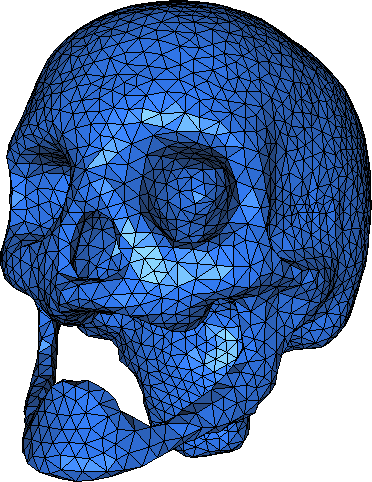
\includegraphics[height=10cm]{Surface_mesher/skull-surface}
%\end{center}
%\end{ccTexOnly}
%\begin{ccHtmlOnly}
%<img border="0" src="./skull-surface.png" align="center" height="75%">
%\end{ccHtmlOnly}

\begin{center}
 \begin{ccTexOnly}
   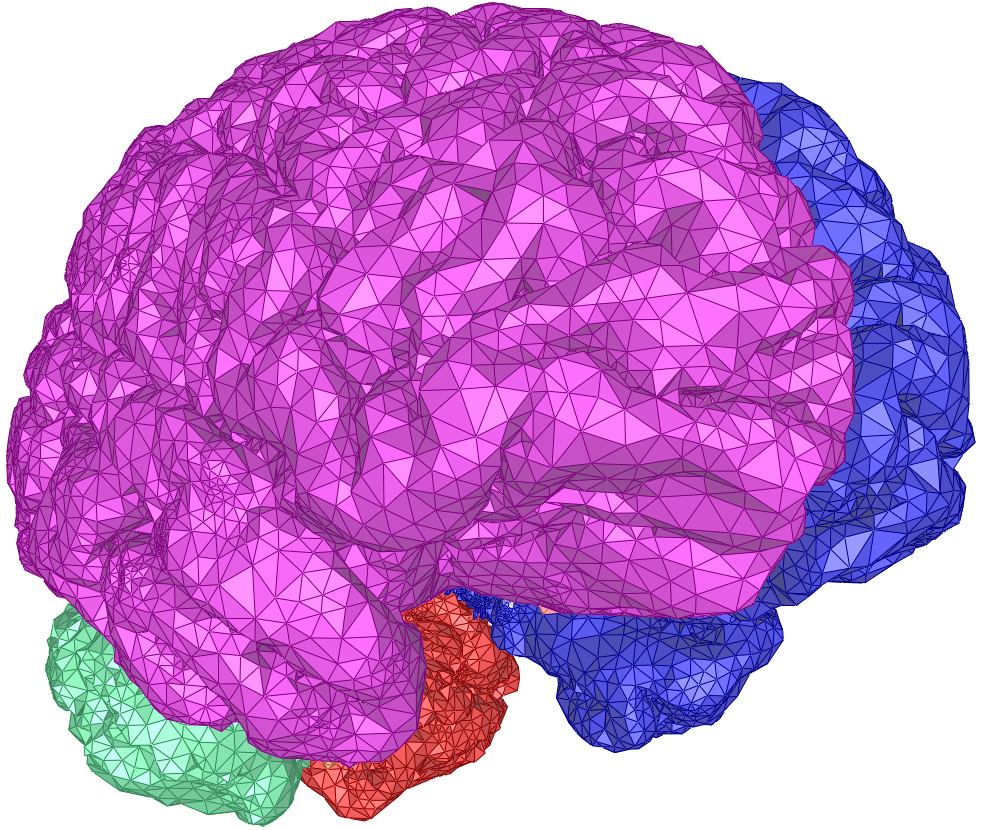
\includegraphics[height=10cm]{Surface_mesher/segmented_head}
 \end{ccTexOnly}
 \begin{ccHtmlOnly}
   <img border="0" src="./segmented_head.png">
 \end{ccHtmlOnly}
\end{center}

\section{Introduction\label{SurfaceMesher_section_intro}}

This package provides a function template
to compute a triangular mesh approximating a surface.

The meshing algorithm requires to know the surface to be meshed
only  through an oracle able to  tell whether a
given segment, line or ray intersects the surface or not
and to compute an intersection point if any.
This feature makes the package generic enough to be
applied in a wide variety of situations. For instance, it can be
used to mesh implicit surfaces described as the zero level set
of some function. It may also be used in the field of medical imaging
to mesh surfaces described as a gray
level set in a three dimensional image.

The surface is required to be either a smooth surface, with a continuous
field of normal unitary vectors, or a piecewise-smooth surface, where the
set of discontinuity points of the normals field is the union of a set of
smooth curves. These smooth curves are called the \emph{1D curves} of the surface.

If the surface contains 1D curves, the knowledge of these curves is only
given by an oracle, able to tell if a given triangle intersects one of
these curves, and compute an intersection point if any.


The meshing algorithm is based on the notion of the restricted
Delaunay triangulation. Basically the algorithm  computes a set of
sample points on the surface, and extract an interpolating 
surface mesh  from the three dimensional triangulation of these 
sample points. 
%It also interpolates a 1D mesh of the 1D curves of the
%surface, if any.
Points are iteratively added to the sample,
as in a Delaunay refinement process, until some size and shape
criteria on the elements of the surface mesh 
%and the 1D mesh
are satisfied. 


The size and shape criteria guide the  behavior of
the refinement process and control its termination.
They also condition  the size and shape of the elements in the final
mesh. Naturally, those criteria can be customized to satisfy
the user needs. The \ccc{Surface mesh generation} package offers
a set of standard criteria that can be scaled through
three numerical values. Also the user can also plug in its own 
set of refinement criteria.

There is no restriction on the topology and number of components
of the surface provided that the oracle (or the user)
is able to provide one initial sample point on each connected component.
If the surface is smooth enough, and if the size criteria are
small enough, the algorithm guarantees 
that the output mesh is homeomorphic to the
surface, and  is within a small bounded distance
(Hausdorff or even Frechet distance) from the surface.
The algorithm can also be used for non smooth surfaces
but then there is no guarantee. 




\section{The Surface Mesh Generator Interface for Smooth Surfaces\label{SurfaceMesher_section_interface}}
\def\ccLongParamLayout{\ccTrue}
The meshing process is launched through a call to a function template.
There are two overloaded versions of the meshing function
whose signatures are the following:

\ccGlobalFunction{template <class SurfaceMeshC2T3,
                            class Surface,
                            class FacetsCriteria,
                            class Tag >
void make_surface_mesh(SurfaceMeshC2T3& c2t3,
                       Surface surface,
                       FacetsCriteria criteria,
                       Tag ) ;}


\ccGlobalFunction{template <class SurfaceMeshC2T3,
                            class SurfaceMeshTraits,
                            class FacetsCriteria,
                            class Tag >
void make_surface_mesh(SurfaceMeshC2T3& c2t3,
                       SurfaceMeshTraits::Surface_3  surface,
		       SurfaceMeshTraits traits,
                       FacetsCriteria criteria,
                       Tag );}



The template parameter \ccc{SurfaceMeshC2T3} 
stands for  a  data structure type  that is used
to store  the surface mesh.  This type is required to be
a model of the concept \ccc{SurfaceMeshComplex_2InTriangulation_3}.
Such a data structure 
has a pointer to a three dimensional triangulation and encodes
the surface mesh as a subset of facets in this triangulation.
%The data structure is described in the concept
%\ccc{SurfaceMeshComplex_2InTriangulation_3} 
%which is a specialized version
%of a more general concept called  \ccc{Complex_2InTriangulation_3}.
%More precisely, the concept \ccc{Complex_2InTriangulation_3}
%encodes a two dimensional complex embedded  in a three dimensional
%triangulation, which means that the faces of the complex form a subset
%of the triangulation faces. The concept \ccc{PureComplex_2InTriangulation_3} is 
%specialized to the case where the complex is pure which means that it
%is a set of facets (i.e., two dimensional faces) with  their subfaces.
An argument of type  \ccc{SurfaceMeshC2T3} is passed by reference to the meshing
function. This argument holds the output mesh at the end of the
process.

The template parameter \ccc{Surface}  stands for the surface type.
This type has to be a model of the concept \ccc{Surface_3}.

The knowledge on the surface, required by the surface mesh generator
is  encapsulated in a
traits class. Actually, the mesh generator accesses the surface to be meshed
through this traits class only. 
The traits class is required to be a model
of the concept \ccc{SurfaceMeshTraits_3}. 
The difference between the two overloaded versions of
\ccc{make_surface_mesh}
can be explained as follows
\begin{itemize}
\item
In the first  overloaded version
of \ccc{make_surface_mesh},  the surface type  is given  
as template parameter  (\ccc{Surface}) and the \ccc{surface}
to be meshed is passed as parameter to the mesh generator.
In that case the surface mesh generator traits type 
is  automatically generated form the surface type
by an auxiliary class called  the \ccc{Surface_mesh_traits_generator_3}.
  %through
%the class 
%\ccc{Surface_mesh_traits_generator_3<Surface>}.
%(This mechanism is similar to the 
%\ccc{Kernel_traits}  mechanism.) \\
\item In the second overloaded version of \ccc{make_surface_mesh}, 
the surface mesh generator traits type is provided
by the  template parameter \ccc{SurfaceMeshTraits_3}
and the surface type is obtained from this traits type.
Both  a surface and a traits 
are passed to the mesh generator as arguments. 
\end{itemize}


The first overloaded version can be used
whenever the surface type either provides  a nested type
\ccc{Surface::Surface_mesher_traits_3} 
that is  a model of \ccc{SurfaceMeshTraits_3}
or is a surface type for which a specialization
of the traits generator \ccc{Surface_mesh_traits_generator_3<Surface>}
is provided.
Currently, the library provides partial specializations
of  \ccc{Surface_mesher_traits_generator_3<Surface>}
for implicit surfaces (\ccc{Implicit_surface_3<Traits, Function>}) and 
gray level images (\ccc{Gray_level_image_3<FT, Point>}).



The parameter \ccc{criteria} handles the description of the size and shape
criteria driving the meshing process. The template parameter \ccc{FacetsCriteria}
has to be instantiated by a model of the concept \ccc{SurfaceMeshFacetsCriteria}.


The parameter \ccc{Tag}  is a tag 
whose type influences the behavior of the
meshing algorithm. For instance, this parameter
can be used to enforce the manifold property
of the output mesh while avoiding 
an over-refinement of the mesh. Further details on this
subject are given in 
Section~\ref{SurfaceMesher_section_variations}.

A call to 
\ccc{make_surface_mesh(c2t3,surface, criteria, tag)} launches 
the meshing process with an initial 
set of points which is the union of two subsets:
the set of vertices in the  initial triangulation pointed to by \ccc{c2t3},
and a set of points provided by the \ccc{Compute_initial_points()} functor 
of the traits class. This initial set of points is required 
to include at least one point on each connected component of the surface
to be meshed.


% \section{The Surface Mesh Generator Interface for Piecewise Smooth
%   Surfaces\label{SurfaceMesher_piecewise_section_interface}}

% The meshing process for piecewise smooth surfaces is launched in a way
% similar to the smooth case. There are also two overloaded versions of a
% meshing function:

% \ccGlobalFunction{template <class SurfaceMeshC2T3,
%                             class Surface,
%                             class FacetsCriteria,
%                             class EdgesCriteria,
%                             class Tag >
% void make_piecewise_smooth_surface_mesh(SurfaceMeshC2T3& c2t3,
%                                         Surface surface,
%                                         FacetsCriteria facets_criteria,
%                                         EdgesCriteria edges_criteria
%                                         Tag ) ;}


% \ccGlobalFunction{template <class SurfaceMeshC2T3,
%                             class SurfaceMeshTraits,
%                             class FacetsCriteria,
%                             class EdgesCriteria,
%                             class Tag >
% void make_piecewise_smooth_surface_mesh(SurfaceMeshC2T3& c2t3,
%                                         SurfaceMeshTraits::Surface_3  surface,
% 		                        SurfaceMeshTraits traits,
%                                         FacetsCriteria facets_criteria,
%                                         EdgesCriteria edges_criteria
%                                         Tag );}


% Every parameters has the same meaning than in the smooth case. The template
% parameter \ccc{SurfaceMeshTraits} has to be a model of the concept
% \ccc{PiecewiseSmoothSurfaceMeshTraits_3}, which refines the concept
% \ccc{SurfaceMeshTraits_3} by adding the methods needed to compute the
% intersections between a triangle and the set of 1D curves of the piecewise
% smooth surface \ccc{surface}.

% The parameter \ccc{edges_criteria} gives the size criteria on the edges of
% the 1D mesh interpolating the 1D curves.

\def\ccLongParamLayout{\ccFalse}

\section{Examples}
\label{SurfaceMesher_section_example}


\subsection{Meshing an Implicit Surface}

The first code example meshes a sphere 
given as the zero level set of a function $\R^3 \longrightarrow \R$.
More precisely, 
the surface to be meshed is created 
by the constructor
of the class \ccc{Implicit_surface_3<Kernel, Function>}
from a pointer to the function (\ccc{sphere_function})
and a bounding sphere.

The default meshing criteria are determined  by three numerical
values: 
\begin{itemize}
\item \ccc{angular_bound} is a lower bound in degrees for the angles 
     of mesh facets.
\item \ccc{radius_bound} is an upper bound on the radii of surface Delaunay
balls. A surface Delaunay ball is a ball circumscribing a mesh facet
and centered on the surface. 
\item \ccc{distance_bound} is an upper bound for the distance 
between the circumcenter of a mesh facet and the center of a surface
Delaunay ball of this facet.
\end{itemize}

Given this surface type, the surface mesh generator will use
an automatically generated traits class.

The resulting mesh is shown in 
Figure~\ref{figure:Surface_mesher-sphere-surface}.

\begin{figure}[ht]
  \begin{center}
    \begin{ccTexOnly}
      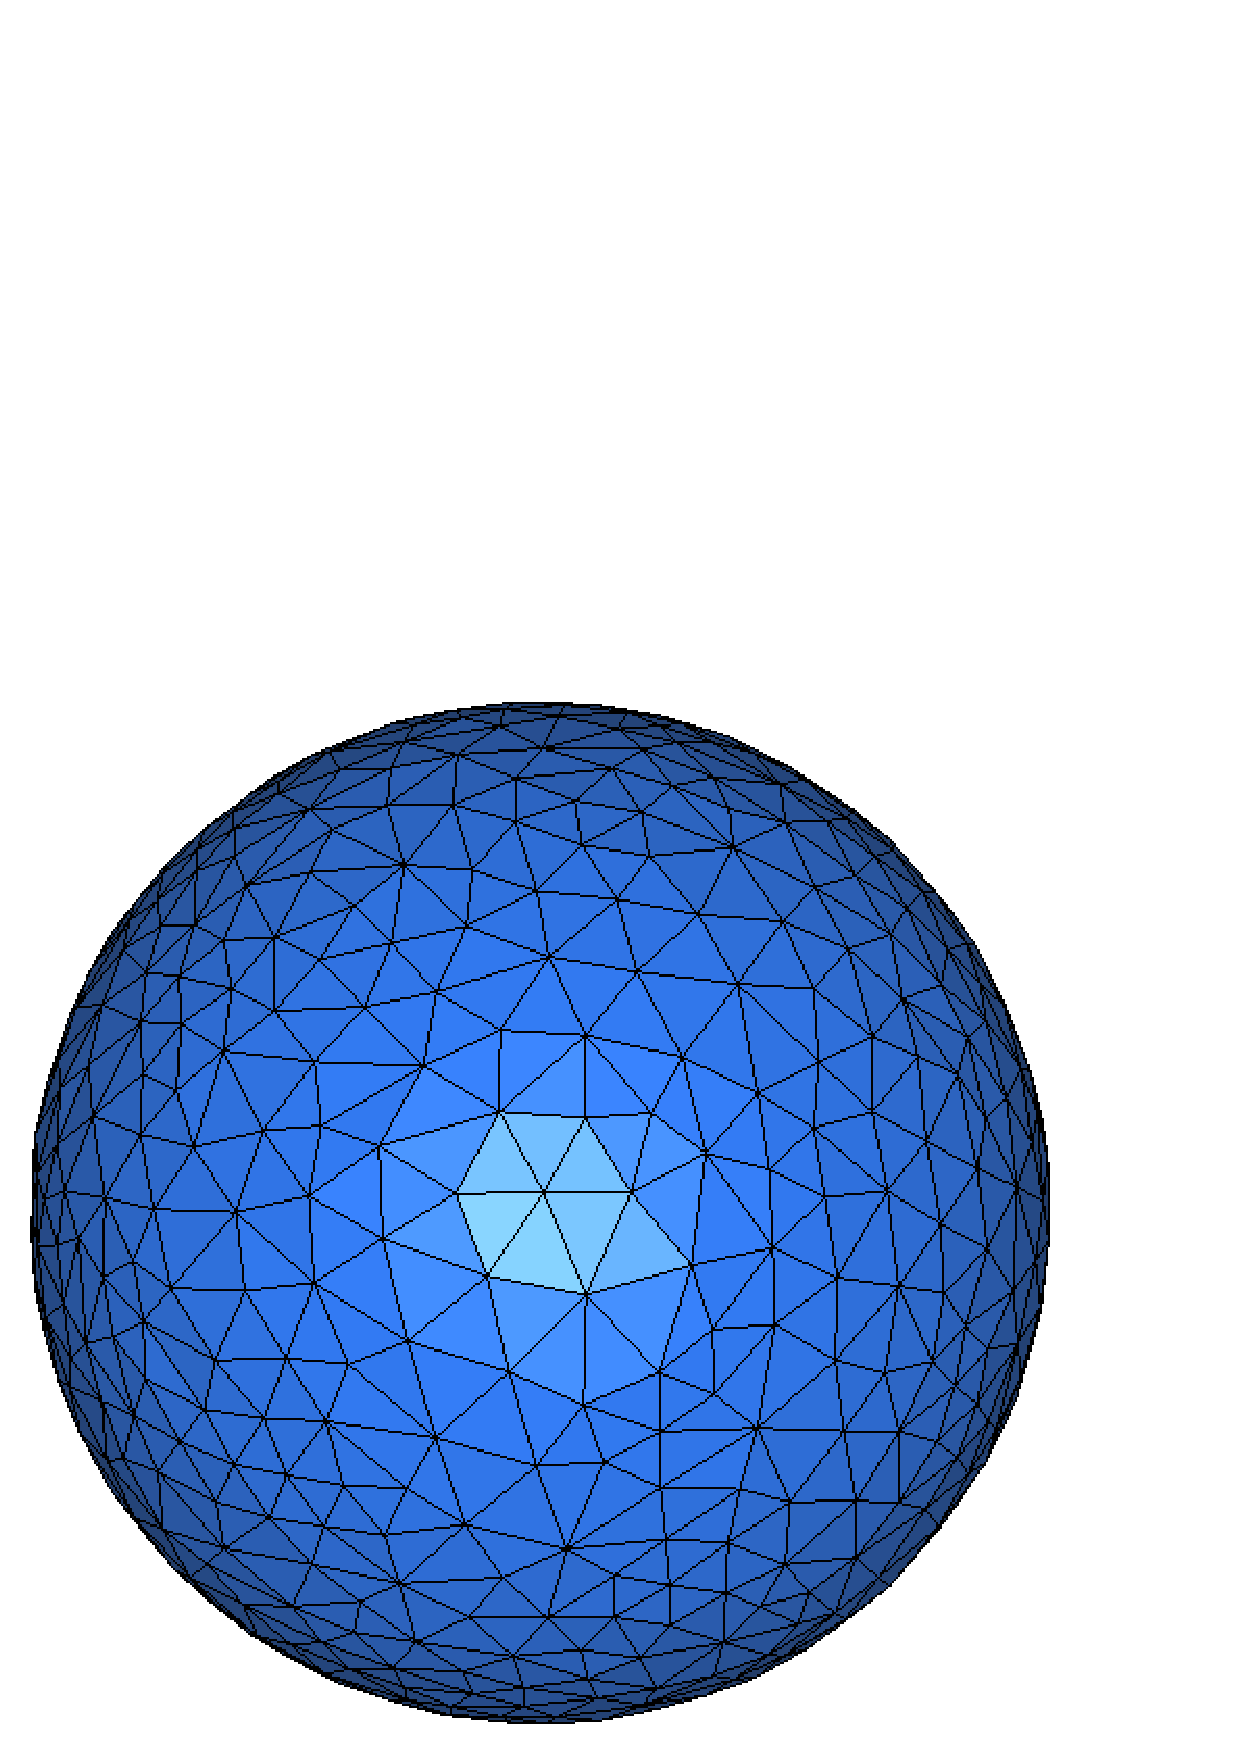
\includegraphics[height=10cm]{Surface_mesher/sphere-surface}
    \end{ccTexOnly}
    \begin{ccHtmlOnly}
      <img border="0" src="./sphere-surface.png" height="75%">
    \end{ccHtmlOnly}
  \end{center}
  \caption{Surface mesh of a sphere}
  \label{figure:Surface_mesher-sphere-surface}
\end{figure}

\ccIncludeExampleCode{Surface_mesher/mesh_an_implicit_function.cpp}

\subsection{Meshing a Surface Defined as a Gray Level in a 3D Image}
In this example the surface to be meshed is defined
as the locus of points with a given gray level
in a 3D image.
The code is quite similar to the previous example. 

The main difference with the previous code 
is that the function used to define the surface
is  an object of type  \ccc{CGAL::Gray_level_image_3} created from
an image file and a numerical value that is  the
 gray value of the level one wishes to mesh.

Note that  surface, which is still an object of type  \ccc{Implicit_surface_3}
is now, defined by three parameters that are the function, the bounding
sphere and a numerical value called {\em the precision}. This
precision, whose value
is relative to the bounding sphere radius, is used in the intersection
computation.
This parameter has a default which was used in the previous example.
Also note that the center of the bounding sphere is required to be
internal a point where the function has a negative value.

The chosen iso-value of this 3D~image corresponds to a head skull. The
resulting mesh is shown in Figure~\ref{figure:Surface_mesher-skull}.

\begin{figure}[ht]
  \begin{center}
    \begin{ccTexOnly}
      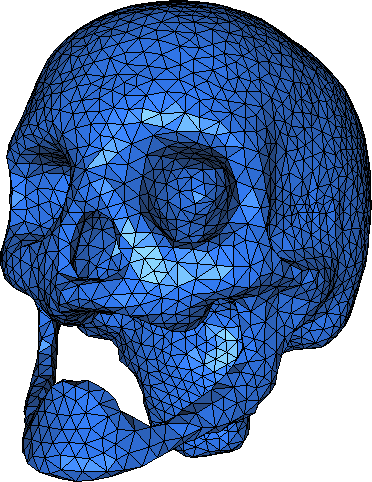
\includegraphics[height=10cm]{Surface_mesher/skull-surface}
    \end{ccTexOnly}
    \begin{ccHtmlOnly}
      <img border="0" src="./skull-surface.png" height="75%">
    \end{ccHtmlOnly}
  \end{center}
  \caption{Surface mesh of an iso-contour extracted from a gray level 3D~image}
  \label{figure:Surface_mesher-skull}
\end{figure}

\ccIncludeExampleCode{Surface_mesher/mesh_a_3d_gray_image.cpp}

% \subsection{Remeshing a polyhedral surface}
% In this example, the surface is a polyhedral surface, that represents a
% piecewise smooth surface. The 1D curves of that surfaces are the union o
% the border edges (if any) and the edges at which the dihedral angle is
% smaller than 120~degrees. The polyhedral surface is given by an OFF file.

% The criteria on the facets of the surface mesh are given by the same class
% than in the smooth case. Some extra criteria on the edges of the 1D mesh
% are given.

% \ccIncludeExampleCode{Surface_mesher/polyhedron_remesher.cpp}

\section{Meshing Criteria, Guarantees and Variations\label{SurfaceMesher_section_criteria}}
\label{SurfaceMesher_section_variations}

The guarantees on the output mesh depend on the mesh criteria.
Theoretical guarantees are given in \cite{cgal:bo-pgsms-05}.
First, the meshing algorithm is proved to terminate 
if the angular bound is
not smaller than $30$~degrees. 
Furthermore, the output mesh 
is guaranteed to be homeomorphic to the surface,
and  there is a guaranteed bound 
on the  distance (Hausdorff and even Frechet distance)
between the mesh and the surface
if the radius bound is everywhere smaller than 
the $\epsilon$ times the local feature size. 
Here $\epsilon$ is a constant that has to be
less than 0.16, and the local feature size 
$lfs(x)$ is defined on each point $x$ of the surface
as the distance from $x$ to the medial axis.  
Note that the radius bound need not be uniform,
although it is a uniform bound in the default criteria.

Naturally, such a theoretical guarantee can be only achieved
for smooth surfaces that have a finite, non zero
reach value. (The reach of a surface is the minimum value 
of local feature size on
this surface).

The value of the local feature size on any point of the surface
or its minimum on the surface it usually unknown
although it can sometimes be guessed. Also it happens frequently
that setting the meshing criteria so as to fulfill the theoretical
conditions yields an over refined mesh.
On the other hand, when the size criteria are relaxed,
no homeomorphism with the input surface is guaranteed,
and the output mesh is not even guaranteed to be manifold.
To remedy this problem and give a more flexible
meshing algorithm, the function template
\ccc{make_surface_mesh} has a tag template parameter
allowing to slightly change the behavior of the refinement process.
This feature allows, for instance,  to run the meshing
algorithm with a relaxed size criteria, more coherent
with the size of the mesh expected by the user,
and still have a guarantee that
the output mesh forms a manifold surface.
The function \ccc{make_surface_mesh} has specialized versions
for the following  tag types: \\
\ccc{Manifold_tag}: the output mesh is guaranteed to be a manifold
surface without boundary.\\
\ccc{Manifold_with_boundary_tag}: the output mesh is guaranteed to be
manifold but may have boundaries.\\
\ccc{Non_manifold_tag}: the algorithm relies on the given criteria and
guarantees nothing else.

\section{Undocumented features available in demos}

The Polyhedron demo has a feature that allows to remesh a polyhedral
surface, using the 3D Surface Mesh Generator. That has been implemented as
a special model of \ccc{SurfaceMeshTraits_3}, for polyhedra. That traits
class is not yet documented because its interface and code have not yet
been stabilized. It will probably be shipped with next release of CGAL.

The Surface Mesh Generator demo allows to mesh not only gray level images,
but also segmented images, when voxels are labelled with a domain
index. Such images are for example the result of a segmentation of 3D
medical images. This feature is not yet ready to be documented in current
release, but will probably be in next release of CGAL.

\section{Design and Implementation History}

The algorithm implemented in this package
is mainly based on the  work of Boissonnat and Oudot
\cite{cgal:bo-pgsms-05}

The meshing algorithm is implemented using the design of mesher levels
described in \cite{cgal:ry-gsddrm-06}. 

David Rey, Steve Oudot and Andreas Fabri have participated
in the development of this package.




